\documentclass[11pt,a4paper]{article}
\usepackage[margin=2.3cm]{geometry}
\usepackage[T1]{fontenc}
\usepackage{lmodern}
\usepackage{microtype}
\usepackage{xspace}
\usepackage{booktabs}
\usepackage{tabularx}
\usepackage{array}
\usepackage{graphicx}
\usepackage{float}
\usepackage{xcolor}
\usepackage{enumitem}
\usepackage{caption}
\usepackage{titlesec}
\usepackage{fancyhdr}
\usepackage[hidelinks]{hyperref}

\definecolor{rmblue}{HTML}{2B6CB0}
\definecolor{rmorange}{HTML}{DD6B20}
\definecolor{rmgrey}{HTML}{4A5568}

% auto-generated by make_numbers.py -- do not edit
\newcommand{\ResRawMain}{2,484\xspace}
\newcommand{\ResRawUpd}{962\xspace}
\newcommand{\ResRaw}{3,446\xspace}
\newcommand{\ResEmpty}{1\xspace}
\newcommand{\ResMojibake}{38\xspace}
\newcommand{\ResNonEn}{0\xspace}
\newcommand{\ResExactDup}{798\xspace}
\newcommand{\ResExactDupUpd}{796\xspace}
\newcommand{\ResNearDup}{8\xspace}
\newcommand{\ResShort}{27\xspace}
\newcommand{\ResLong}{27\xspace}
\newcommand{\ResIQR}{222\xspace}
\newcommand{\ResJunk}{7\xspace}
\newcommand{\ResPlow}{97\xspace}
\newcommand{\ResPhigh}{2,047\xspace}
\newcommand{\ResPII}{117\xspace}
\newcommand{\ResPIItokens}{299\xspace}
\newcommand{\ResFinal}{2,632\xspace}
\newcommand{\ResFinalMain}{2,473\xspace}
\newcommand{\ResFinalUpd}{159\xspace}
\newcommand{\ResCats}{24\xspace}
\newcommand{\JobRawLI}{33,246\xspace}
\newcommand{\JobRawRZ}{352\xspace}
\newcommand{\JobRaw}{33,598\xspace}
\newcommand{\JobEmpty}{1\xspace}
\newcommand{\JobNonEn}{23\xspace}
\newcommand{\JobExactDup}{3,236\xspace}
\newcommand{\JobNearDup}{2,087\xspace}
\newcommand{\JobShort}{280\xspace}
\newcommand{\JobLong}{283\xspace}
\newcommand{\JobIQR}{532\xspace}
\newcommand{\JobJunk}{165\xspace}
\newcommand{\JobPlow}{42\xspace}
\newcommand{\JobPhigh}{1,331\xspace}
\newcommand{\JobPII}{4,818\xspace}
\newcommand{\JobFinal}{28,086\xspace}
\newcommand{\JobFinalLI}{27,738\xspace}
\newcommand{\JobFinalRZ}{348\xspace}
\newcommand{\JobSalaryShare}{39.8\xspace}
\newcommand{\JobSenUnknown}{7,927\xspace}
\newcommand{\JobSenMissPct}{27.3\xspace}
\newcommand{\FitPairsTrain}{6,241\xspace}
\newcommand{\FitPairsTest}{1,759\xspace}
\newcommand{\EscoSkills}{13,896\xspace}
\newcommand{\EscoAlt}{99,192\xspace}
\newcommand{\RozeeQueries}{19\xspace}
\newcommand{\RozeeQueriesDefined}{33\xspace}
\newcommand{\RozeeRequests}{556\xspace}
\newcommand{\RozeeBlocked}{87\xspace}
\newcommand{\RozeeDelay}{0\xspace}
\newcommand{\SkillVocab}{1,169\xspace}
\newcommand{\TfidfVocab}{50,000\xspace}
\newcommand{\MeanSkillsRes}{7.95\xspace}
\newcommand{\MeanSkillsJob}{3.91\xspace}
\newcommand{\YearsCovRes}{95.8\xspace}
\newcommand{\YearsCovJob}{46.9\xspace}
\newcommand{\JobCatCov}{60.9\xspace}
\newcommand{\ResTrain}{1,842\xspace}
\newcommand{\ResVal}{395\xspace}
\newcommand{\ResTest}{395\xspace}
\newcommand{\JobTrain}{19,660\xspace}
\newcommand{\JobVal}{4,213\xspace}
\newcommand{\JobTest}{4,213\xspace}
\newcommand{\Pairs}{15,755\xspace}
\newcommand{\PairsPos}{7,859\xspace}
\newcommand{\PairsHard}{5,264\xspace}
\newcommand{\PairsRand}{2,632\xspace}
\newcommand{\PairsTrain}{11,052\xspace}
\newcommand{\PairsVal}{2,351\xspace}
\newcommand{\PairsTest}{2,352\xspace}
\newcommand{\CosPos}{0.12\xspace}
\newcommand{\CosHard}{0.13\xspace}
\newcommand{\CosRand}{0.03\xspace}
\newcommand{\RefYear}{2019\xspace}
\newcommand{\ImbalanceRatio}{9.91\xspace}
\newcommand{\MedWordsRes}{745\xspace}
\newcommand{\MedWordsJob}{444\xspace}
\newcommand{\SkillsUniqJobs}{2,278\xspace}
\newcommand{\SkillsUniqRes}{1,505\xspace}
\newcommand{\SkillsOverlap}{1,302\xspace}
\newcommand{\SkillsJobOnly}{976\xspace}
\newcommand{\SkillsJaccard}{0.53\xspace}
\newcommand{\TopHundredMissing}{22\xspace}
\newcommand{\AucTfidf}{0.40\xspace}
\newcommand{\AucEmb}{0.53\xspace}
\newcommand{\EmbPos}{0.48\xspace}
\newcommand{\EmbHard}{0.46\xspace}
\newcommand{\CorrYearsSalary}{0.54\xspace}
\newcommand{\CorrWordsSkillsJob}{0.48\xspace}
\newcommand{\CorrWordsSkillsRes}{0.42\xspace}
\newcommand{\RozeeMale}{7\xspace}
\newcommand{\RozeeFemale}{1\xspace}
\newcommand{\RozeeGendered}{8\xspace}
\newcommand{\RozeeTopSkills}{artificial intelligence, Python, computer science, Git, CI/CD\xspace}
\newcommand{\ResCatMin}{BPO\xspace}
\newcommand{\ResCatMinN}{22\xspace}
\newcommand{\ResCatMax}{IT\xspace}
\newcommand{\ResCatMaxN}{218\xspace}

% auto-generated by make_tables.py -- do not edit
\newcommand{\BiPreAucHard}{0.539\xspace}
\newcommand{\BiPrePthree}{0.429\xspace}
\newcommand{\BiPreAuc}{0.644\xspace}
\newcommand{\BiAucHard}{0.724\xspace}
\newcommand{\BiPthree}{0.631\xspace}
\newcommand{\BiAuc}{0.801\xspace}
\newcommand{\BiBestEpoch}{3\xspace}
\newcommand{\BiEpochs}{3\xspace}
\newcommand{\BiTriplets}{1,842\xspace}
\newcommand{\BiRuns}{5\xspace}
\newcommand{\BiBestLr}{$1\times10^{-4}$\xspace}
\newcommand{\BiBestBs}{32\xspace}
\newcommand{\BiBestLen}{256\xspace}
\newcommand{\MnALr}{$1\times10^{-3}$\xspace}
\newcommand{\MnABs}{64\xspace}
\newcommand{\MnADrop}{0.3\xspace}
\newcommand{\MnAHidden}{256\xspace}
\newcommand{\MnAEpoch}{14\xspace}
\newcommand{\MnAValAuc}{0.860\xspace}
\newcommand{\MnAParams}{412,385\xspace}
\newcommand{\MnAAblPre}{0.783\xspace}
\newcommand{\MnAAblNoFeat}{0.834\xspace}
\newcommand{\MnBLr}{$1\times10^{-3}$\xspace}
\newcommand{\MnBBs}{64\xspace}
\newcommand{\MnBDrop}{0.5\xspace}
\newcommand{\MnBHidden}{128\xspace}
\newcommand{\MnBEpoch}{26\xspace}
\newcommand{\MnBValAuc}{0.807\xspace}
\newcommand{\MnBParams}{202,273\xspace}
\newcommand{\MnBAblPre}{0.820\xspace}
\newcommand{\MnBAblNoFeat}{0.800\xspace}
\newcommand{\MnRuns}{36\xspace}
\newcommand{\ResAF}{0.784\xspace}
\newcommand{\ResAP}{0.705\xspace}
\newcommand{\ResAR}{0.883\xspace}
\newcommand{\ResAAuc}{0.862\xspace}
\newcommand{\ResAAucLo}{0.85\xspace}
\newcommand{\ResAAucHi}{0.88\xspace}
\newcommand{\ResAAtsAuc}{0.588\xspace}
\newcommand{\ResAAtsF}{0.665\xspace}
\newcommand{\ResAPreAuc}{0.661\xspace}
\newcommand{\ResABiAuc}{0.790\xspace}
\newcommand{\ResAGbAuc}{0.832\xspace}
\newcommand{\ResALrAuc}{0.808\xspace}
\newcommand{\ResAN}{2,352\xspace}
\newcommand{\ResAPosShare}{50\xspace}
\newcommand{\ResAFP}{431\xspace}
\newcommand{\ResAFN}{136\xspace}
\newcommand{\ResBF}{0.737\xspace}
\newcommand{\ResBP}{0.668\xspace}
\newcommand{\ResBR}{0.822\xspace}
\newcommand{\ResBAuc}{0.768\xspace}
\newcommand{\ResBAucLo}{0.74\xspace}
\newcommand{\ResBAucHi}{0.79\xspace}
\newcommand{\ResBAtsAuc}{0.536\xspace}
\newcommand{\ResBAtsF}{0.678\xspace}
\newcommand{\ResBPreAuc}{0.579\xspace}
\newcommand{\ResBBiAuc}{0.633\xspace}
\newcommand{\ResBGbAuc}{0.695\xspace}
\newcommand{\ResBLrAuc}{0.648\xspace}
\newcommand{\ResBN}{1,759\xspace}
\newcommand{\ResBPosShare}{51\xspace}
\newcommand{\ResBFP}{369\xspace}
\newcommand{\ResBFN}{161\xspace}
\newcommand{\AccPos}{0.883\xspace}
\newcommand{\AccHard}{0.510\xspace}
\newcommand{\AccRand}{0.889\xspace}
\newcommand{\FitNo}{0.344\xspace}
\newcommand{\FitPot}{0.634\xspace}
\newcommand{\FitGood}{0.687\xspace}
\newcommand{\AucGoodNo}{0.788\xspace}
\newcommand{\PthreeTfidf}{0.406\xspace}
\newcommand{\PthreePre}{0.417\xspace}
\newcommand{\PthreeFt}{0.634\xspace}
\newcommand{\PthreeRerank}{0.641\xspace}
\newcommand{\PthreeRandom}{0.050\xspace}
\newcommand{\PthreeWorst}{Agriculture (0.00), Automobile (0.00), BPO (0.08)\xspace}
\newcommand{\PthreeBest}{Chef (1.00), HR (0.98), Accountant (0.96)\xspace}
\newcommand{\ErrWorst}{\emph{pending}\xspace}
\newcommand{\ErrBest}{\emph{pending}\xspace}
\newcommand{\ErrHard}{\emph{pending}\xspace}
\newcommand{\ErrPos}{\emph{pending}\xspace}
\newcommand{\ErrRand}{\emph{pending}\xspace}
\newcommand{\ErrPot}{\emph{pending}\xspace}
\newcommand{\ErrNoFit}{\emph{pending}\xspace}
\newcommand{\ErrGood}{\emph{pending}\xspace}
\newcommand{\ErrStatus}{pending\xspace}
\newcommand{\BiasN}{300\xspace}
\newcommand{\BiasConclusion}{\emph{pending}\xspace}


\setlist{nosep,leftmargin=1.4em}
\captionsetup{font=small,labelfont=bf}
\titleformat{\section}{\large\bfseries\color{rmblue}}{\thesection}{0.8em}{}
\titleformat{\subsection}{\normalsize\bfseries}{\thesubsection}{0.6em}{}
\newcommand{\phase}[1]{\vspace{0.6em}\noindent{\Large\bfseries\color{rmgrey}#1}\par\vspace{0.2em}\noindent\textcolor{rmgrey}{\rule{\linewidth}{0.6pt}}\par\vspace{0.3em}}
\newcommand{\code}[1]{\texttt{\small #1}}
\newcolumntype{L}{>{\raggedright\arraybackslash}X}

\pagestyle{fancy}
\fancyhf{}
\fancyhead[L]{\small\textcolor{rmgrey}{Resumatch --- Deliverable 3}}
\fancyhead[R]{\small\textcolor{rmgrey}{AI Semester Project, FAST-NUCES Lahore}}
\fancyfoot[C]{\small\thepage}
\renewcommand{\headrulewidth}{0.4pt}

\begin{document}

\begin{titlepage}
\centering
{\large FAST National University of Computer and Emerging Sciences, Lahore\par}
\vspace{0.3em}
{\normalsize Artificial Intelligence --- Semester Project\par}
\vspace{4.5em}
{\fontsize{40}{46}\selectfont\bfseries\color{rmblue} Resumatch\par}
\vspace{0.6em}
{\Large AI-Powered Resume--Job Matching Platform\par}
\vspace{3em}
{\large\bfseries Deliverable 3: Final Deployment \& Technical Report\par}
\vspace{0.4em}
{\normalsize Phases 1--6 --- Track A, Application Development\par}
\vspace{4em}
\begin{tabular}{ll}
\toprule
\textbf{Member} & \textbf{Roll No. / Section}\\
\midrule
Muhammad Sufyan & 24L-2601 / BSDS-5B\\
Muaaz Fahad & 24L-2563 / BSDS-5B\\
Hanan Ishaque & 24L-2537 / BSDS-5B\\
\bottomrule
\end{tabular}
\vspace{2.5em}
{\normalsize\url{https://github.com/Suf-7/Resumatch}\par}
\vspace{0.4em}
{\normalsize\url{https://huggingface.co/Suf7/resumatch-models}\par}
\vfill
{\large November 2026\par}
\end{titlepage}

\tableofcontents
\thispagestyle{fancy}
\newpage

\section{Abstract}
Resumatch is a resume--job matching application for the Pakistani market. A job seeker uploads a
CV and receives the three best Rozee.pk postings they can apply to, each with an apply link, a
learned MatchNet score, a rule-based ATS score and an explicit skill-gap list. Recruiters paste a
job description and a batch of CVs and get a ranked shortlist.

We collected and cleaned \ResFinal resumes and \JobFinal postings, built \Pairs weakly labelled
pairs and an open-jobs pool with apply URLs. Matching uses a two-stage PyTorch stack: a fine-tuned
MiniLM bi-encoder for retrieval and MatchNet, a small MLP over embedding interactions plus ten
interpretable features, for re-ranking. On occupation-level (weak) test pairs MatchNet reaches
AUC-ROC \ResAAuc and F1 \ResAF; on external human-labelled fit pairs it reaches AUC-ROC \ResBAuc
and F1 \ResBF, beating a rule-based ATS score, TF-IDF, pretrained MiniLM and gradient boosting.
Hard negatives (related occupations) remain the main failure mode (error rate \ErrHard). A
counterfactual bias check on 300 pairs shows at most 1.7\% of decisions flip when gender, name
origin or university is swapped. The hosted Streamlit app (\code{app/streamlit\_app.py}) serves
both user modes with the trained weights from Hugging Face.

\phase{Phase 1: Problem Definition}

\section{Problem and Product}
Hiring is a two-sided matching problem. Candidates often send one generic CV and never learn why
they were filtered; recruiters face more applications than they can read. Keyword ATS tools reward
stuffing and miss capable people who phrase skills differently. Our data confirms a vocabulary
gap: \SkillsJobOnly of the \SkillsUniqJobs distinct skills in postings never appear in any resume.

\paragraph{Product.} Track~A application. A candidate uploads a resume and sees the top three
\emph{open} postings with apply links, MatchNet and ATS scores, and matched/missing skills. A
recruiter uploads a job description plus several CVs and gets a ranked shortlist. Matching and
ranking models are trained by us; LLMs are used only for optional labelling and synthetic data.

\paragraph{Audience.} Pakistani graduates and early-career applicants (Rozee.pk), and recruiters
at SMEs who want an explained shortlist rather than a black-box score.

\phase{Phase 2: Data Foundations}

\section{Data Collection and Cleaning}
\begin{itemize}
\item Resumes: Kaggle Resume Dataset + Updated Resume Dataset $\rightarrow$ \ResFinal cleaned
(\ResCats categories), PII masked.
\item Postings: LinkedIn Job Postings 2023--24 (\JobFinalLI, training only) and Rozee.pk
(\JobFinalRZ) with apply URLs and closing dates for the live pool.
\item Skills: ESCO v1.1.2 gazetteer (\EscoSkills skills).
\item External evaluation: human-labelled resume--JD fit pairs (\FitPairsTrain + \FitPairsTest).
\end{itemize}
Cleaning drops empty/non-English text, repairs encoding, removes exact and near-duplicates
(TF-IDF $> 0.95$), handles length outliers and masks email, phone and URLs. Features (train-only
fit): TF-IDF, multi-hot skills, years of experience, standardized numerics, MiniLM embeddings.
Splits are 70/15/15 \emph{by resume and by posting}. Pairs: \PairsPos same-category positives,
\PairsHard hard negatives, \PairsRand random negatives.

\begin{figure}[H]
\centering
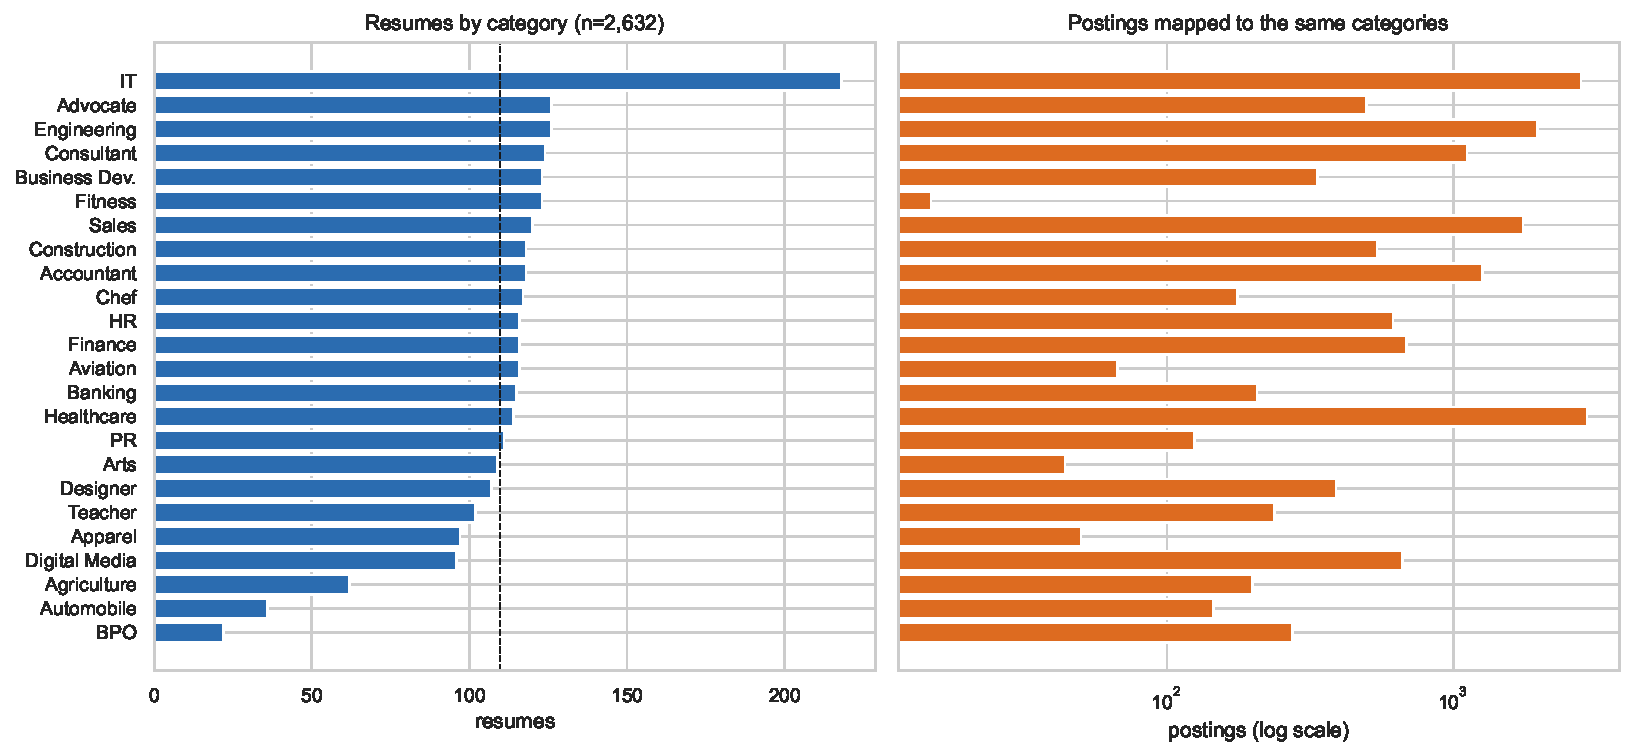
\includegraphics[width=0.86\linewidth]{figures/fig_category_distribution.pdf}
\caption{Resume and posting category distributions after cleaning.}
\end{figure}

\begin{figure}[H]
\centering
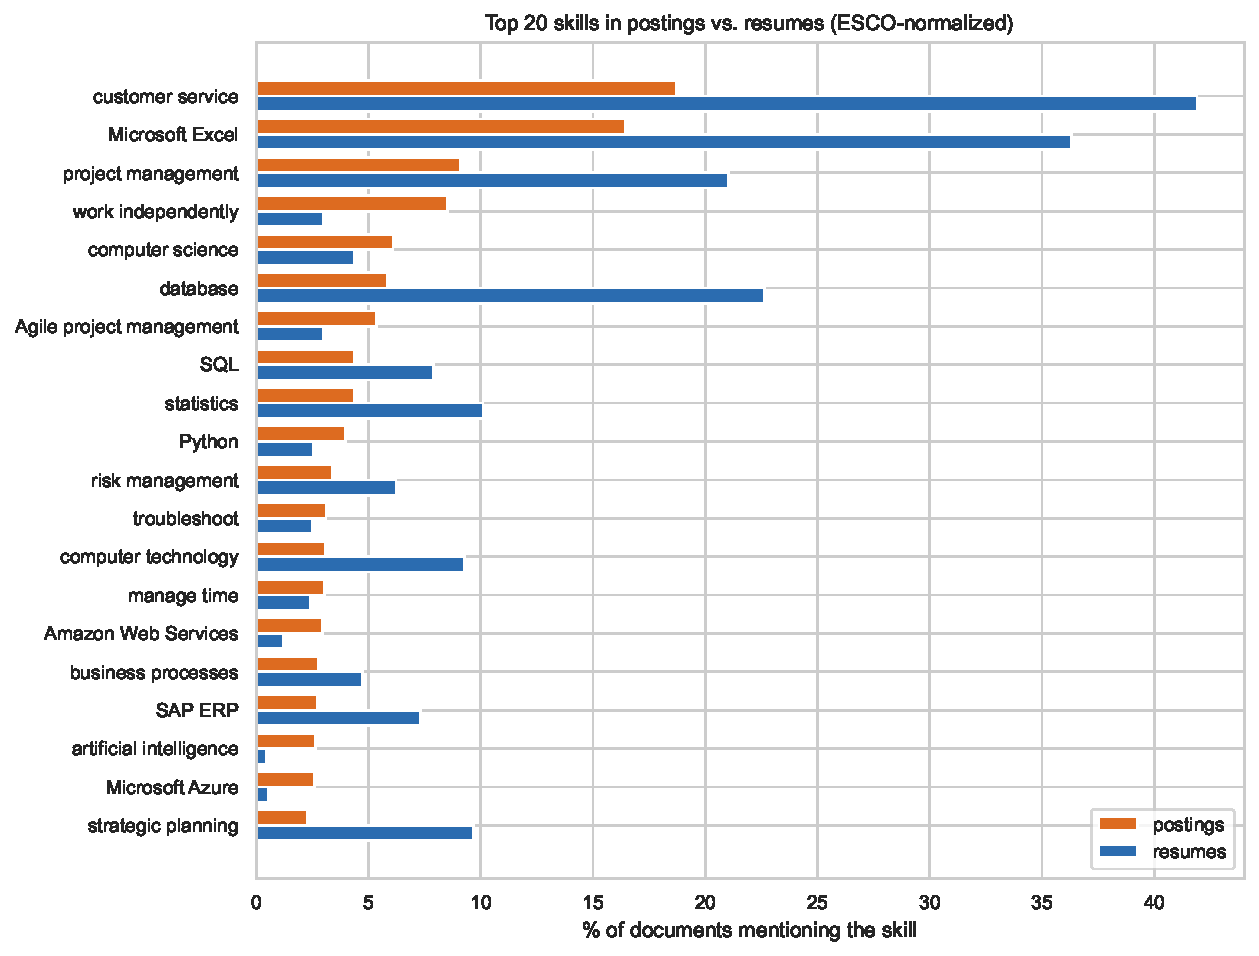
\includegraphics[width=0.92\linewidth]{figures/fig_top_skills.pdf}
\caption{Top skills in postings versus resumes: resumes over-emphasize generic skills.}
\end{figure}

The baseline ATS score (skills 0.50, experience 0.20, title 0.15, structure 0.15) reaches AUC
\AtsAucRand against random negatives but only \AtsAucHard against hard negatives --- so a learned
ranker is necessary.

\phase{Phase 3: Model Architecture \& Training}

\section{Two-Stage Matcher}
\begin{figure}[H]
\centering
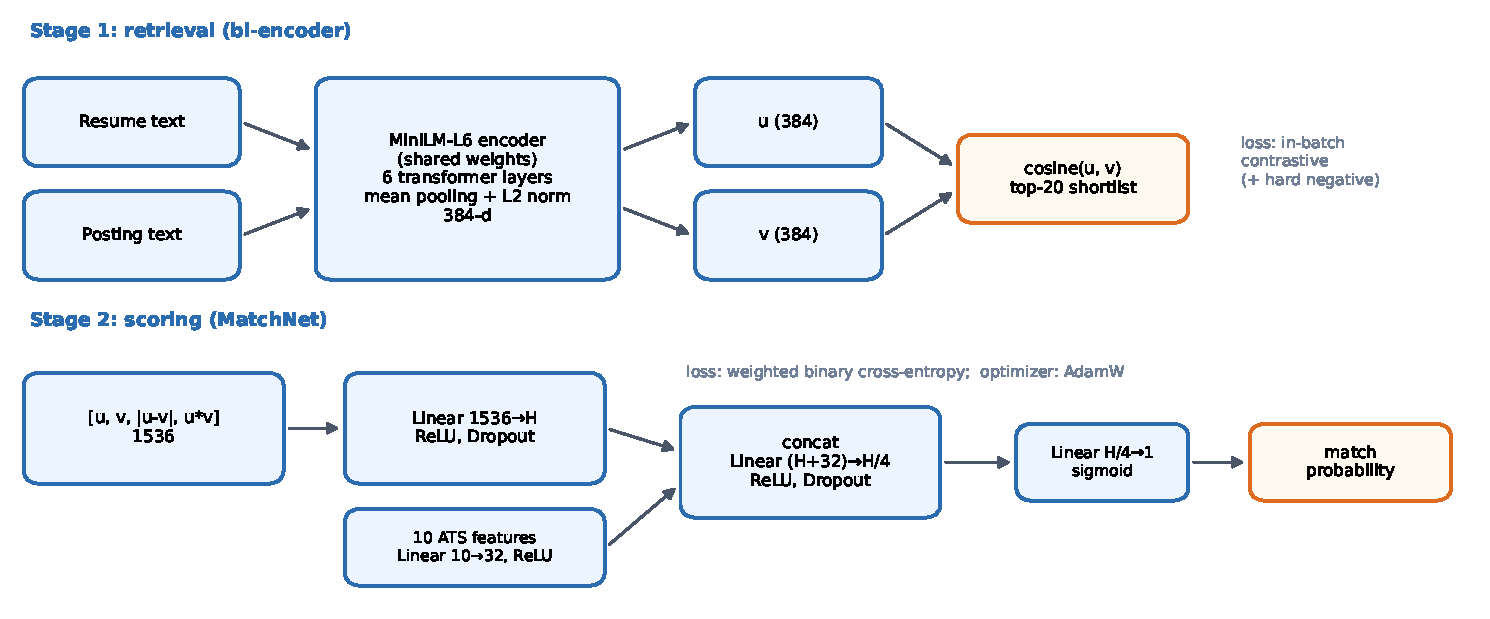
\includegraphics[width=\linewidth]{figures/fig_architecture.pdf}
\caption{Stage~1 bi-encoder retrieval; Stage~2 MatchNet re-ranking with ATS features.}
\end{figure}

\paragraph{Bi-encoder.} \code{all-MiniLM-L6-v2} (6 layers, 384-d, mean pool, L2). Loss: multiple-
negatives ranking with in-batch negatives plus one mined hard negative (scale 20). Optimizer:
AdamW, 10\% warm-up, linear decay, grad clip 1.0. Selected: lr \BiBestLr, batch \BiBestBs, length
\BiBestLen (val AUC-hard \BiAucHard, P@3 \BiPthree).

\paragraph{MatchNet.} Input $[u,v,|u-v|,u \odot v]$ plus ten scalar features
$\rightarrow$ Linear--ReLU--Dropout branches $\rightarrow$ logit. Loss: class-weighted BCE.
Optimizer: AdamW, early stop on val AUC (patience 6). Selected Task~A: lr \MnALr, batch \MnABs,
dropout \MnADrop, $H=\MnAHidden$ (val AUC \MnAValAuc). Task~B: lr \MnBLr, batch \MnBBs, dropout
\MnBDrop, $H=\MnBHidden$ (val AUC \MnBValAuc).

\begin{table}[H]
\centering\small
\begin{tabularx}{\linewidth}{@{}c c c c r r r r@{}}
\toprule
Learning rate & Batch & Max len & Best ep. & Val AUC & Val AUC (hard) & Val P@3 & Min\\
\midrule
\multicolumn{4}{l}{pretrained MiniLM, no fine-tuning} & 0.644 & 0.539 & 0.429 & --\\
$1\times10^{-5}$ & 32 & 256 & 3 & 0.729 & 0.628 & 0.544 & 8\\
$3\times10^{-5}$ & 32 & 256 & 3 & 0.771 & 0.683 & 0.609 & 8\\
\textbf{$1\times10^{-4}$} & \textbf{32} & \textbf{256} & \textbf{3} & \textbf{0.801} & \textbf{0.724} & \textbf{0.631} & \textbf{8}\\
$3\times10^{-5}$ & 16 & 256 & 3 & 0.793 & 0.714 & 0.629 & 9\\
$3\times10^{-5}$ & 32 & 128 & 3 & 0.751 & 0.666 & 0.579 & 3\\
\bottomrule
\end{tabularx}
\caption{Bi-encoder hyperparameter search (validation split). Selection criterion: AUC of positives vs.\ hard negatives. The selected run is in bold.}\label{tab:bigrid}
\end{table}

\begin{table}[H]
\centering\small
\begin{tabularx}{\linewidth}{@{}l c c c@{}}
\toprule
Hyperparameter & Value & Task A: mean / max val AUC & Task B: mean / max val AUC\\
\midrule
Learning rate & $1\times10^{-4}$ & 0.835 / 0.839 & 0.773 / 0.781\\
 & $3\times10^{-4}$ & 0.841 / 0.847 & 0.781 / 0.793\\
 & $1\times10^{-3}$ & \textbf{0.853 / 0.860} & \textbf{0.794 / 0.807}\\
\addlinespace
Batch size & 64 & \textbf{0.845 / 0.860} & \textbf{0.787 / 0.807}\\
 & 256 & 0.840 / 0.857 & 0.779 / 0.800\\
\addlinespace
Dropout & 0.1 & 0.841 / 0.858 & 0.780 / 0.795\\
 & 0.3 & \textbf{0.843 / 0.860} & 0.781 / 0.807\\
 & 0.5 & 0.845 / 0.858 & \textbf{0.788 / 0.807}\\
\addlinespace
Hidden size $H$ & 128 & 0.842 / 0.855 & \textbf{0.784 / 0.807}\\
 & 256 & \textbf{0.844 / 0.860} & 0.782 / 0.806\\
\bottomrule
\end{tabularx}
\caption{MatchNet grid search: all 36 combinations of the values below were trained per task; each cell averages (and maximizes) validation AUC over the runs with that value. Bold marks the value of the selected configuration. The full grid is in the appendix.}\label{tab:mngrid}
\end{table}


\begin{figure}[H]
\centering
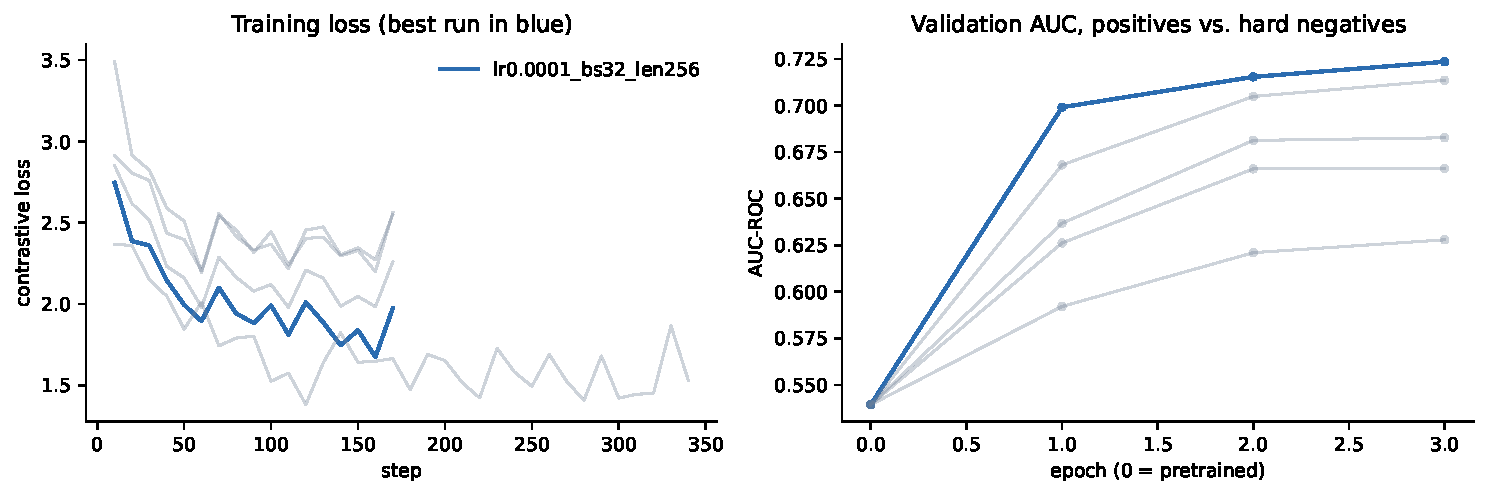
\includegraphics[width=\linewidth]{figures/fig_bi_encoder_curves.pdf}
\caption{Bi-encoder training loss and validation AUC (hard negatives).}
\end{figure}

\begin{figure}[H]
\centering
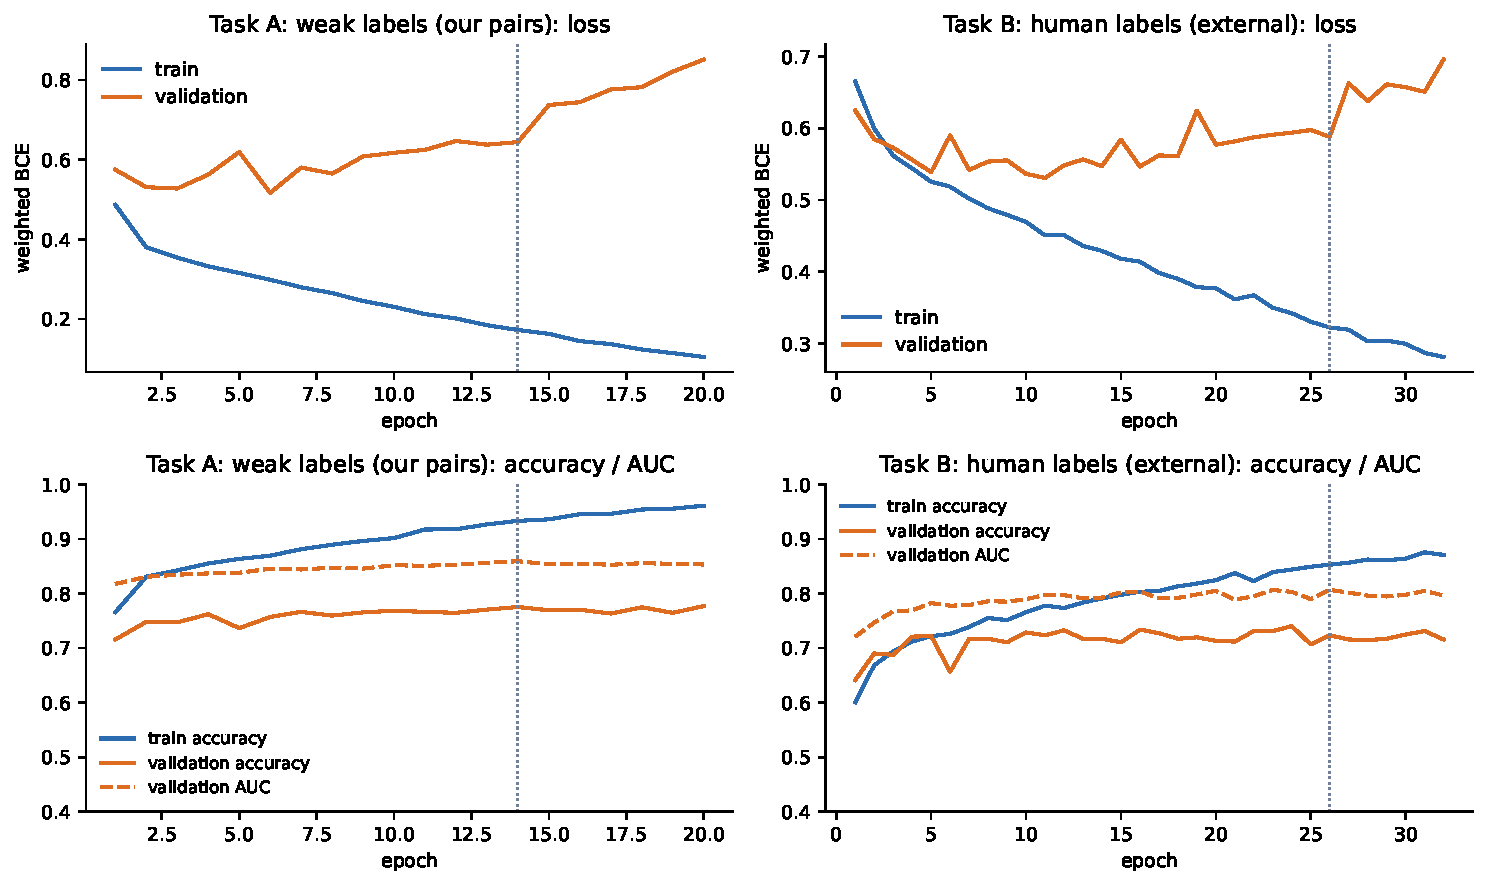
\includegraphics[width=\linewidth]{figures/fig_matchnet_curves.pdf}
\caption{MatchNet loss and accuracy/AUC; dashed line = early-stopping epoch.}
\end{figure}

\phase{Phase 4: Evaluation \& Analysis}

\section{Validation and Metrics}
Fixed entity-level train/val/test (not K-fold): fine-tuning the transformer many times is too
expensive, and with thousands of pairs a held-out split already gives tight bootstrap CIs.
Thresholds maximize validation F1 and are frozen for test. We report Precision, Recall, F1,
AUC-ROC and PR-AUC because the product problem is heavily imbalanced even when our constructed
test splits are near-balanced.

\begin{table}[H]
\centering\small
\begin{tabularx}{\linewidth}{@{}l r r r r r r@{}}
\toprule
Model & Precision & Recall & F1 & Accuracy & AUC-ROC [95\% CI] & PR-AUC\\
\midrule
ATS score (rules) & 0.498 & 0.997 & 0.665 & 0.500 & 0.588 [0.56, 0.61] & 0.563\\
TF-IDF cosine & 0.552 & 0.973 & 0.704 & 0.594 & 0.571 [0.55, 0.59] & 0.555\\
MiniLM cosine (pretrained) & 0.540 & 0.939 & 0.686 & 0.574 & 0.661 [0.64, 0.68] & 0.622\\
Bi-encoder cosine (fine-tuned) & 0.639 & 0.876 & 0.739 & 0.694 & 0.790 [0.77, 0.81] & 0.770\\
Logistic regression & 0.659 & 0.864 & 0.748 & 0.711 & 0.808 [0.79, 0.82] & 0.791\\
Gradient boosting & 0.724 & 0.810 & 0.764 & 0.752 & 0.832 [0.82, 0.85] & 0.818\\
\textbf{MatchNet} & \textbf{0.705} & \textbf{0.883} & \textbf{0.784} & \textbf{0.759} & \textbf{0.862 [0.85, 0.88]} & \textbf{0.855}\\
\bottomrule
\end{tabularx}
\caption{Task A (weak labels): test-set results (n = 2,352, 50\% positive). Thresholds were chosen on the validation split by maximum F1.}\label{tab:resweak}
\end{table}

\begin{table}[H]
\centering\small
\begin{tabularx}{\linewidth}{@{}l r r r r r r@{}}
\toprule
Model & Precision & Recall & F1 & Accuracy & AUC-ROC [95\% CI] & PR-AUC\\
\midrule
ATS score (rules) & 0.514 & 0.997 & 0.678 & 0.516 & 0.536 [0.51, 0.56] & 0.544\\
TF-IDF cosine & 0.574 & 0.784 & 0.663 & 0.591 & 0.612 [0.58, 0.64] & 0.582\\
MiniLM cosine (pretrained) & 0.537 & 0.876 & 0.666 & 0.550 & 0.579 [0.55, 0.61] & 0.592\\
Bi-encoder cosine (fine-tuned) & 0.571 & 0.887 & 0.695 & 0.601 & 0.633 [0.61, 0.66] & 0.607\\
Logistic regression & 0.563 & 0.897 & 0.692 & 0.590 & 0.648 [0.62, 0.67] & 0.622\\
Gradient boosting & 0.594 & 0.876 & 0.708 & 0.630 & 0.695 [0.67, 0.72] & 0.679\\
\textbf{MatchNet} & \textbf{0.668} & \textbf{0.822} & \textbf{0.737} & \textbf{0.699} & \textbf{0.768 [0.74, 0.79]} & \textbf{0.757}\\
\bottomrule
\end{tabularx}
\caption{Task B (human labels): test-set results (n = 1,759, 51\% positive). Thresholds were chosen on the validation split by maximum F1.}\label{tab:reshuman}
\end{table}


\begin{figure}[H]
\centering
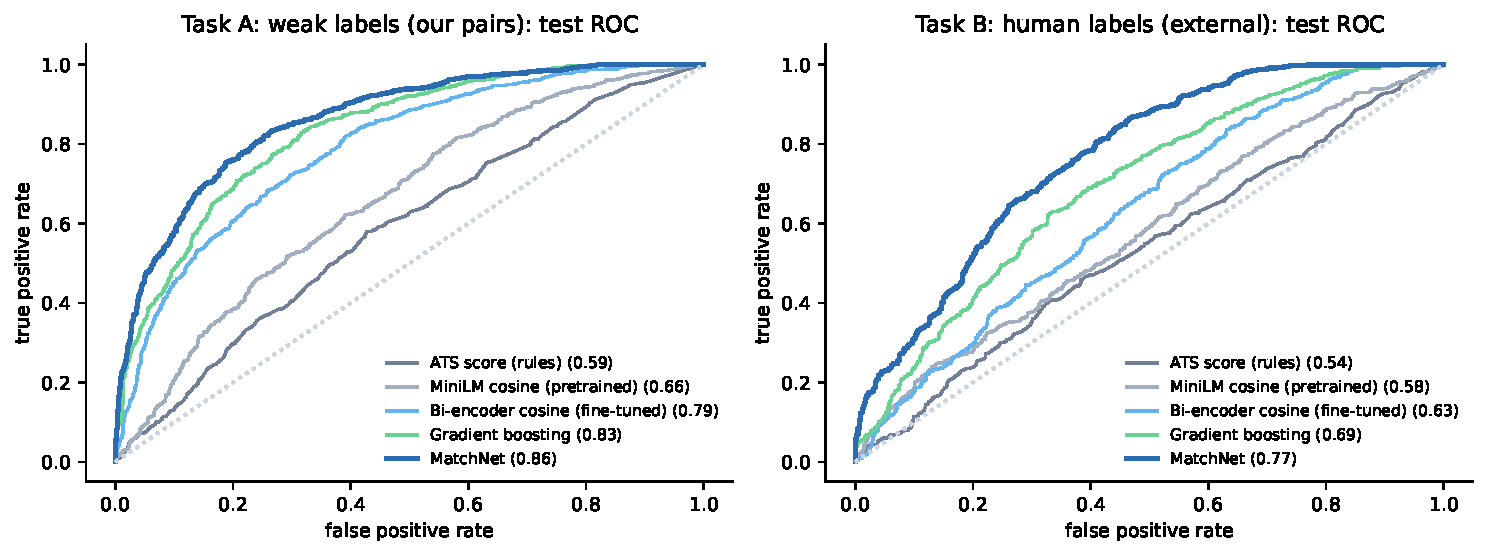
\includegraphics[width=\linewidth]{figures/fig_roc.pdf}
\caption{Test ROC curves for Task~A (left) and Task~B (right).}
\end{figure}

\paragraph{Retrieval.} Precision@3 on the test job pool: pretrained \PthreePre, fine-tuned
\PthreeFt, fine-tuned + MatchNet re-rank \PthreeRerank (random \PthreeRandom).

\begin{table}[H]
\centering\small
\begin{tabularx}{\linewidth}{@{}L r@{}}
\toprule
Ranker & Precision@3\\
\midrule
TF-IDF cosine & 0.406\\
MiniLM (pretrained) & 0.417\\
Bi-encoder (fine-tuned) & 0.634\\
Bi-encoder + MatchNet re-rank & 0.641\\
Random ranking (expected) & 0.050\\
\bottomrule
\end{tabularx}
\caption{Top-3 recommendation on the test split: 395 resumes, each ranked against all 2,565 test postings with a known occupation. A recommended posting counts as relevant if it belongs to the resume's occupation.}\label{tab:retrieval}
\end{table}


\paragraph{Error analysis.} Hard-negative error rate \ErrHard versus \ErrPos on positives and
\ErrRand on random negatives. Worst categories: \ErrWorst; best: \ErrBest. Task~B errors fall with
human grade (No~Fit \ErrNoFit, Potential \ErrPot, Good \ErrGood).

\begin{figure}[H]
\centering
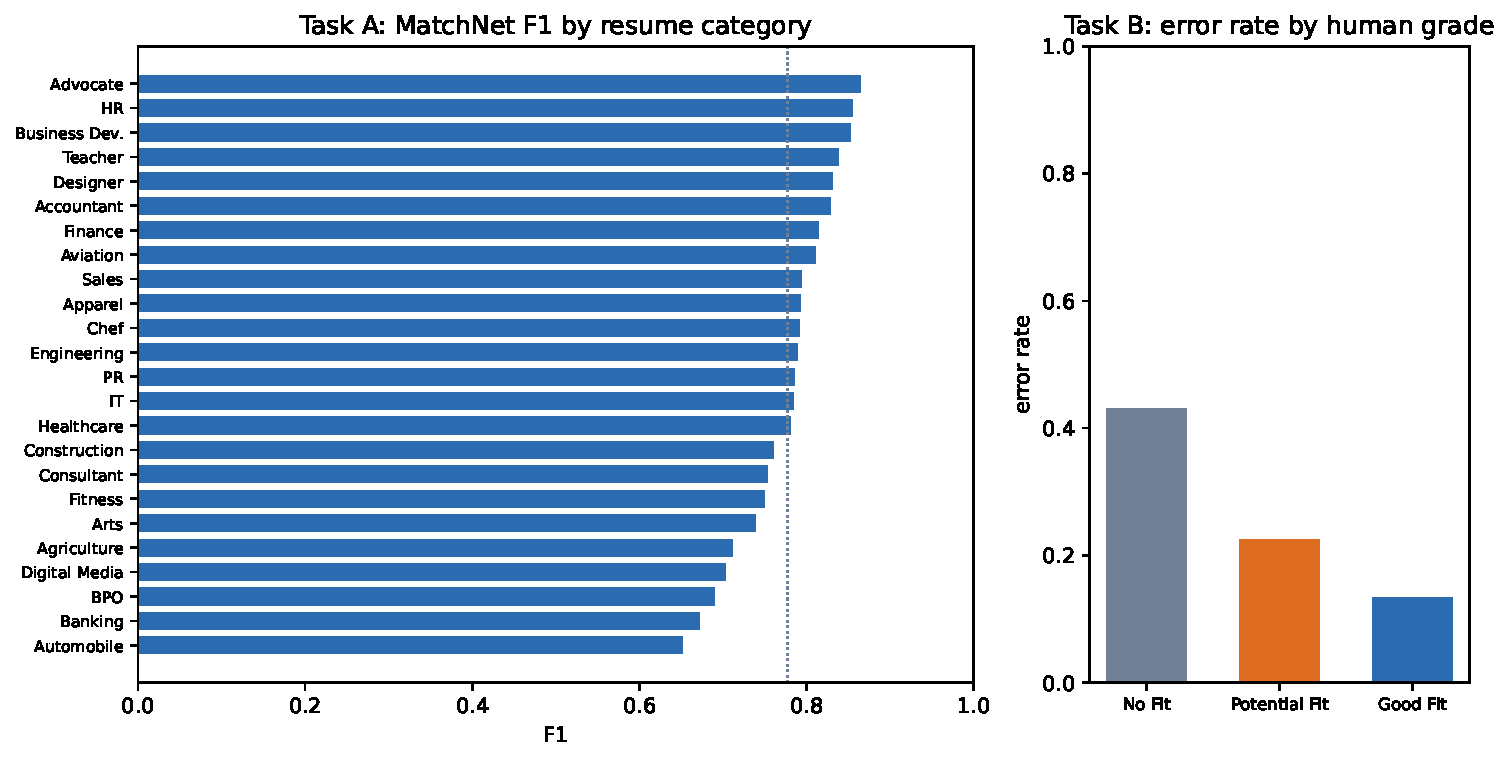
\includegraphics[width=\linewidth]{figures/fig_error_analysis.pdf}
\caption{Per-category F1 (Task~A) and error rate by human grade (Task~B).}
\end{figure}

\paragraph{Bias check.} On \BiasN counterfactual pairs, mean score shifts stay below 0.02 and at
most 1.7\% of decisions flip. \BiasConclusion

\begin{table}[H]
\centering\small
\begin{tabularx}{\linewidth}{@{}L r r r r r@{}}
\toprule
Counterfactual test & Mean $\Delta$ & 95\% CI & Mean $|\Delta|$ & $p$ & Decisions flipped\\
\midrule
gender name & +0.0096 & [+0.0069, +0.0128] & 0.0149 & $<0.001$ & 0.7\%\\
origin name & -0.0142 & [-0.0207, -0.0078] & 0.0274 & $<0.001$ & 1.7\%\\
university & +0.0000 & [-0.0064, +0.0062] & 0.0250 & 0.765 & 1.3\%\\
gender pronoun & +0.0000 & [-0.0000, +0.0001] & 0.0001 & 0.086 & 0.0\%\\
\bottomrule
\end{tabularx}
\caption{Bias check: change in MatchNet score when only one attribute of the resume is swapped (variant B minus variant A).}\label{tab:bias}
\end{table}


\begin{figure}[H]
\centering
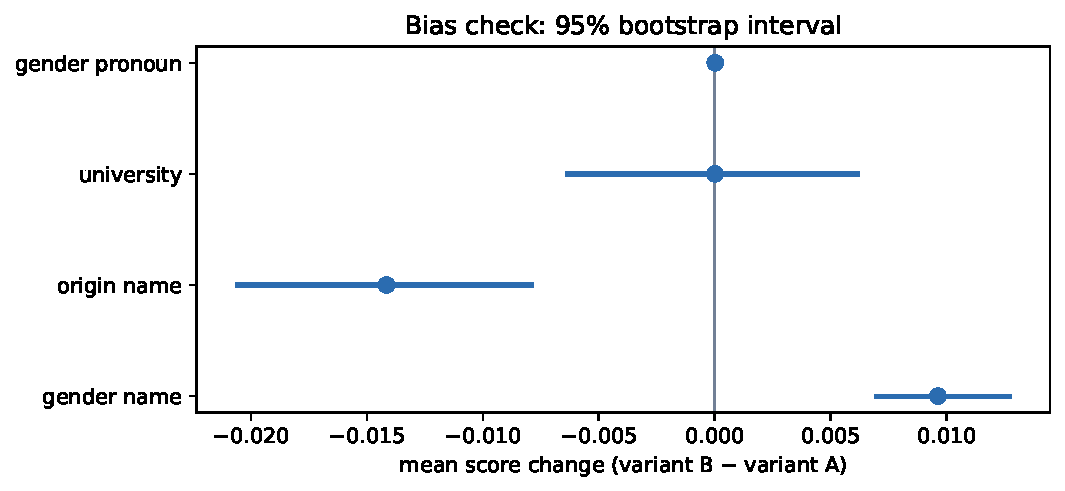
\includegraphics[width=0.82\linewidth]{figures/fig_bias_check.pdf}
\caption{Bias check: mean score change with 95\% bootstrap intervals.}
\end{figure}

\phase{Phase 5: Application}

\section{Streamlit Front End}\label{sec:app}
The production interface is a Streamlit app in \code{app/streamlit\_app.py}. It loads the
fine-tuned bi-encoder and MatchNet once (\code{st.cache\_resource}) and exposes two modes:

\begin{itemize}
\item \textbf{Candidate:} upload a PDF/TXT/DOCX resume (or paste text). The app embeds the resume,
shortlists 20 Rozee.pk postings by cosine similarity, re-ranks with MatchNet and shows the top
three with apply URL, MatchNet \%, ATS score (0--100) and matched/missing skills.
\item \textbf{Recruiter:} paste a job description and upload several resumes; MatchNet ranks the
batch with the same explanations.
\end{itemize}

If every posting in \code{jobs\_live.parquet} has closed, the app falls back to the full scraped
Rozee.pk pool and shows a demo warning; \code{make refresh} updates the pool. Run:

\begin{verbatim}
make weights
.venv/bin/streamlit run app/streamlit_app.py
\end{verbatim}

\begin{figure}[H]
\centering
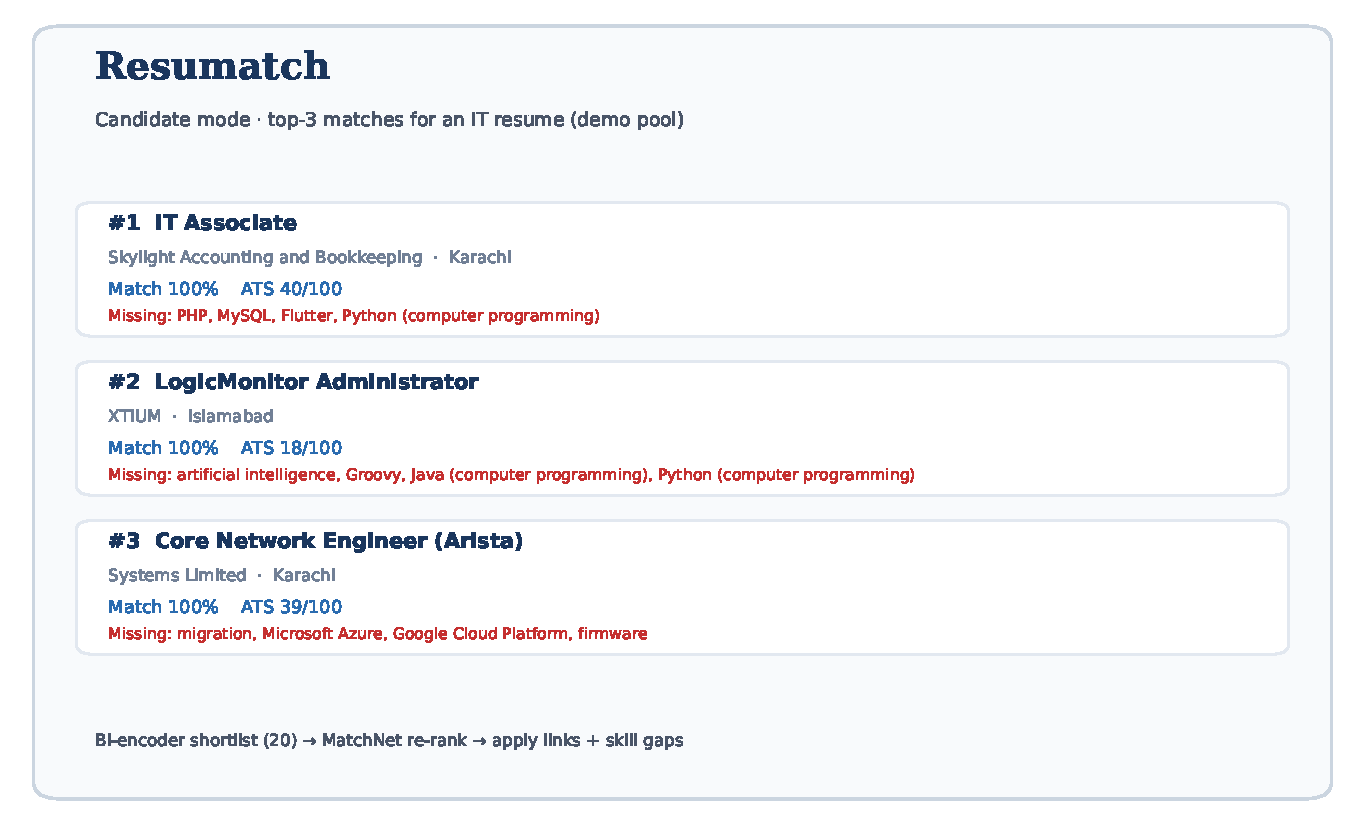
\includegraphics[width=\linewidth]{figures/fig_app_demo.pdf}
\caption{Candidate-mode result card layout: MatchNet and ATS scores, company, and skill gaps
for an IT resume against the Rozee.pk demo pool.}
\end{figure}

\paragraph{Integration.} Inference goes through \code{src/predict.py} (\code{MatchScorer}): the
same code path used in evaluation, so the numbers in Phase~4 and the app stay aligned. PDF text
is extracted with \code{pypdf}; DOCX via the Open XML zip.

\phase{Phase 6: Final Documentation \& Reproducibility}

\section{Limitations}
\begin{itemize}
\item Task~A labels are occupation-level; Task~B is the more honest fit judgement but a single
external dataset.
\item Hard negatives (related occupations) remain near chance for MatchNet.
\item Live postings expire within about a week; the demo pool may show closed apply links until
refreshed.
\item Inputs truncate at \BiBestLen word pieces.
\end{itemize}

\section{Reproducibility}
\begin{itemize}
\item Code: \url{https://github.com/Suf-7/Resumatch} (\code{src/}, \code{app/}, \code{data\_scripts/}).
\item Dependencies: \code{requirements.txt}; \code{make setup}.
\item Weights: \url{https://huggingface.co/Suf7/resumatch-models} via \code{make weights}
(GitHub Release fallback \code{deliverable2-weights}).
\item Train: \code{make train}; evaluate: \code{make evaluate}; this PDF: \code{make report3}.
\end{itemize}

\section{Contribution Table}
\begin{table}[H]
\centering\small
\begin{tabularx}{\linewidth}{@{}l L r r L@{}}
\toprule
Member & Assigned module & Commits & Lines & Main files in git log\\
\midrule
Muhammad Sufyan & \code{src/models/}, \code{train\_*.py}, \code{evaluate.py} & 14 & +5,577 / $-$254 & \code{report (build\_pdf.py)}, \code{README.md}, \code{build\_features.py}, \code{scrape\_jobs.py}\\
Muaaz Fahad & \code{src/error\_analysis.py} & 0 & +0 / $-$0 & ---\\
Hanan Ishaque & \code{src/bias\_check.py} & 0 & +0 / $-$0 & ---\\
\bottomrule
\end{tabularx}
\caption{Contribution table: assigned Deliverable~2 modules, plus Git history from \code{report/contributions.py} (generated files such as figures, PDFs and JSON statistics are excluded).}\label{tab:contrib}
\end{table}


\begin{table}[H]
\centering\small
\begin{tabularx}{\linewidth}{@{}l L@{}}
\toprule
Member & Responsibility across the project\\
\midrule
Muhammad Sufyan & Data pipeline, bi-encoder and MatchNet, evaluation, Streamlit app, reports\\
Muaaz Fahad & Error analysis (\code{src/error\_analysis.py})\\
Hanan Ishaque & Bias check (\code{src/bias\_check.py})\\
\bottomrule
\end{tabularx}
\caption{Module ownership for the final submission.}
\end{table}

\clearpage
\section{Appendix: Full MatchNet Grid}
\begin{table}[H]
\centering\footnotesize
\begin{tabularx}{\linewidth}{@{}c c c c r r r r@{}}
\toprule
LR & Batch & Dropout & $H$ & A: val AUC & A: epoch & B: val AUC & B: epoch\\
\midrule
$1\times10^{-3}$ & 64 & 0.1 & 128 & 0.852 & 14 & 0.793 & 20\\
$1\times10^{-3}$ & 64 & 0.1 & 256 & 0.858 & 14 & 0.795 & 14\\
$1\times10^{-3}$ & 64 & 0.3 & 128 & 0.851 & 16 & 0.807 & 23\\
$1\times10^{-3}$ & 64 & 0.3 & 256 & 0.860 & 14 & 0.796 & 11\\
$1\times10^{-3}$ & 64 & 0.5 & 128 & 0.855 & 23 & 0.807 & 26\\
$1\times10^{-3}$ & 64 & 0.5 & 256 & 0.858 & 14 & 0.806 & 14\\
$1\times10^{-3}$ & 256 & 0.1 & 128 & 0.847 & 29 & 0.782 & 11\\
$1\times10^{-3}$ & 256 & 0.1 & 256 & 0.846 & 30 & 0.780 & 9\\
$1\times10^{-3}$ & 256 & 0.3 & 128 & 0.847 & 31 & 0.786 & 18\\
$1\times10^{-3}$ & 256 & 0.3 & 256 & 0.853 & 31 & 0.789 & 16\\
$1\times10^{-3}$ & 256 & 0.5 & 128 & 0.850 & 31 & 0.800 & 26\\
$1\times10^{-3}$ & 256 & 0.5 & 256 & 0.857 & 38 & 0.793 & 16\\
$3\times10^{-4}$ & 64 & 0.1 & 128 & 0.841 & 31 & 0.785 & 16\\
$3\times10^{-4}$ & 64 & 0.1 & 256 & 0.843 & 31 & 0.779 & 16\\
$3\times10^{-4}$ & 64 & 0.3 & 128 & 0.841 & 27 & 0.783 & 23\\
$3\times10^{-4}$ & 64 & 0.3 & 256 & 0.845 & 31 & 0.778 & 16\\
$3\times10^{-4}$ & 64 & 0.5 & 128 & 0.844 & 31 & 0.793 & 34\\
$3\times10^{-4}$ & 64 & 0.5 & 256 & 0.847 & 36 & 0.787 & 16\\
$3\times10^{-4}$ & 256 & 0.1 & 128 & 0.836 & 59 & 0.778 & 20\\
$3\times10^{-4}$ & 256 & 0.1 & 256 & 0.837 & 46 & 0.770 & 20\\
$3\times10^{-4}$ & 256 & 0.3 & 128 & 0.839 & 40 & 0.772 & 32\\
$3\times10^{-4}$ & 256 & 0.3 & 256 & 0.838 & 37 & 0.771 & 26\\
$3\times10^{-4}$ & 256 & 0.5 & 128 & 0.841 & 59 & 0.786 & 50\\
$3\times10^{-4}$ & 256 & 0.5 & 256 & 0.840 & 38 & 0.784 & 44\\
$1\times10^{-4}$ & 64 & 0.1 & 128 & 0.836 & 58 & 0.776 & 31\\
$1\times10^{-4}$ & 64 & 0.1 & 256 & 0.836 & 51 & 0.773 & 20\\
$1\times10^{-4}$ & 64 & 0.3 & 128 & 0.836 & 51 & 0.772 & 34\\
$1\times10^{-4}$ & 64 & 0.3 & 256 & 0.837 & 40 & 0.773 & 25\\
$1\times10^{-4}$ & 64 & 0.5 & 128 & 0.839 & 59 & 0.774 & 35\\
$1\times10^{-4}$ & 64 & 0.5 & 256 & 0.838 & 40 & 0.781 & 52\\
$1\times10^{-4}$ & 256 & 0.1 & 128 & 0.831 & 59 & 0.777 & 51\\
$1\times10^{-4}$ & 256 & 0.1 & 256 & 0.831 & 59 & 0.773 & 38\\
$1\times10^{-4}$ & 256 & 0.3 & 128 & 0.832 & 60 & 0.771 & 55\\
$1\times10^{-4}$ & 256 & 0.3 & 256 & 0.833 & 59 & 0.771 & 38\\
$1\times10^{-4}$ & 256 & 0.5 & 128 & 0.833 & 60 & 0.767 & 59\\
$1\times10^{-4}$ & 256 & 0.5 & 256 & 0.835 & 59 & 0.774 & 51\\
\bottomrule
\end{tabularx}
\caption{Full MatchNet grid (validation AUC and early-stopped epoch per task).}\label{tab:mnfull}
\end{table}


\begin{thebibliography}{9}\small
\bibitem{kaggle-resume} snehaanbhawal. \emph{Resume Dataset}. Kaggle.
\bibitem{kaggle-linkedin} arshkon. \emph{LinkedIn Job Postings (2023--2024)}. Kaggle.
\bibitem{hf-fit} \emph{resume-job-description-fit}. Hugging Face Datasets.
\bibitem{esco} European Commission. \emph{ESCO} v1.1.2.
\bibitem{sbert} N.~Reimers and I.~Gurevych. Sentence-BERT. \emph{EMNLP}, 2019.
\end{thebibliography}

\end{document}
